\subsubsection{Annif} \label{subject_indexing_annif}

Annif \cite{suominen2019annif} is a tool for automatically indexing subjects to a text. Once trained, it receives a document as an input and outputs its most relevant subjects. It is implemented in Flask\footnote{See \url{https://flask.palletsprojects.com/en/1.1.x/}} as a REST API, which allows for its integration in a larger system as a microservice.

\begin{figure}
    \centering
    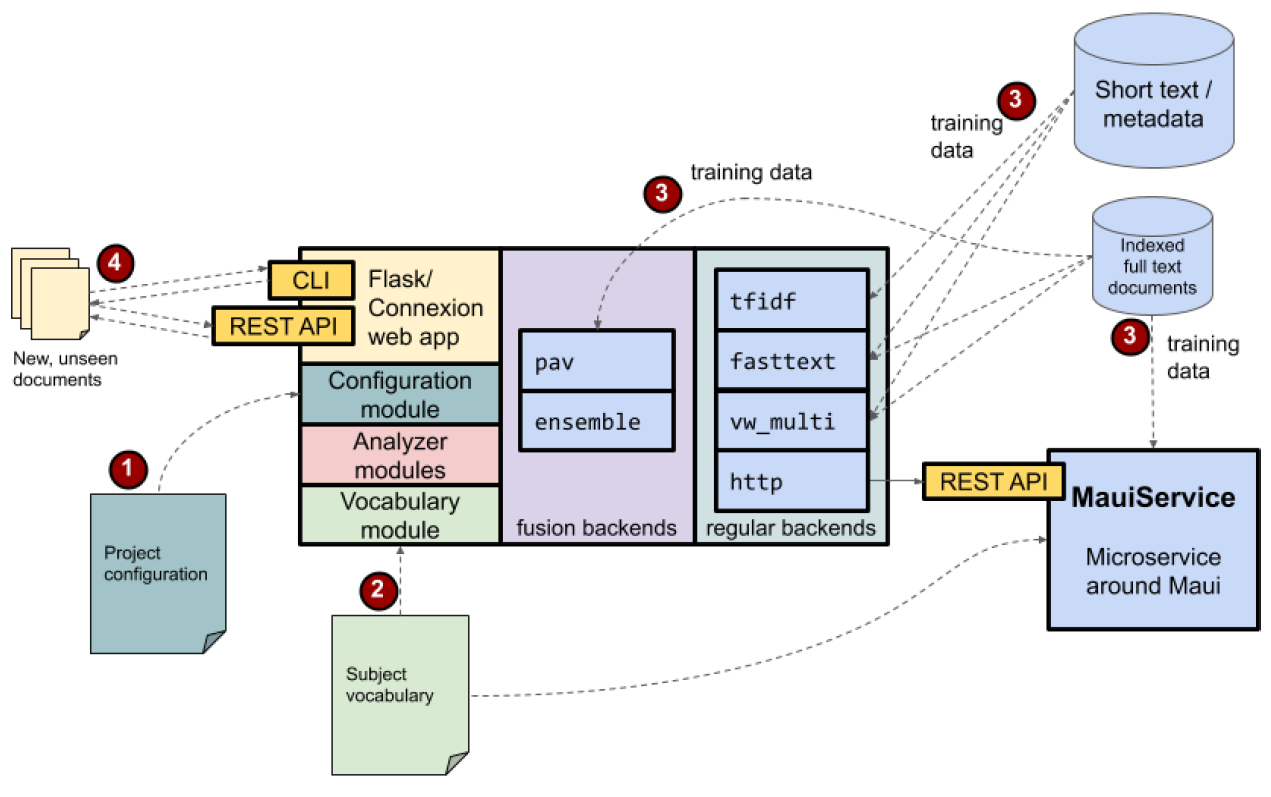
\includegraphics[width=\textwidth]{figures/related_work/annif/annif_architecture.PNG}
    \caption{Annif system architecture}
    \label{fig:annif_architecture}
\end{figure}

\paragraph{Architecture} \mbox{}

Annif's architecture comprises two kinds of components. There are analyzers, which process the input text by performing tokenization and stemming using the NLTK library\footnote{\url{https://www.nltk.org/}}. The analyzers' output is passed onto the backends, which consist of single or a combination of subject indexing algorithms. The authors mention four different algorithms that can be used in Annif:

\begin{enumerate}
    \item \textbf{Maui} incorporates numerous heuristics to match subjects to the frequently occurring or otherwise salient terms in the document. The importance of each heuristic for a given document is determined with a \acrshort{ml} algorithm.
    \item \textbf{TF-IDF} finds correlations between the subjects and a set of representative words of the document. Every subject is associated with a set of words, such as the titles of the documents it appears in. Term frequencies (number of times a term occurs in a document) and inverse document frequencies (inverse fraction of the number of documents that contain a term) are computed for all words appearing in those sets. They are then used to select the most appropriate subjects.
    \item \textbf{fastText} is an \acrshort{ml} algorithm for text classification. Its simple architecture and some other tricks allow it to be trained fast.
    \item \textbf{Vowpal Wabbit} is an online \acrshort{ml} algorithm for multi-class classification.
\end{enumerate}

This architecture follows a modular design which enables adding more analyzers and algorithms. As of today, there are a couple more algorithms available\footnote{Here is the list of available backends:  \url{https://github.com/NatLibFi/Annif/wiki}}, such as STWFSA, based on a finite state automaton and Omikuji, a family of tree-based \acrshort{ml} algorithms.

Annif is able to combine the results of several algorithms by either computing the mean of their predictions or by training a model that maps predictions to subjects using isotonic regression, which estimates the relationship between the score values the algorithms output for each subject and the estimated relevance of the subjects. This latter method was superior to all others, including the individual algorithms. Particularly, it could beat the F1 score (i.e. a weighted average of the precision and recall) of Maui, whose authors state it is as good as humans in the task of subject indexing.

\paragraph{Evaluation} \mbox{}

Unfortunately, the authors mention that Annif's performance is worse in technical fields such as science and technology than in the humanities. They attribute this to the precise definitions of the technical terms when compared to the broader meaning of concepts of the humanities.

Some institutional repositories, such as JYX, from the University of Jyväskylä, have already adopted Annif. JYX uses it to suggest subjects to the student that is submitting a thesis to the repository. After 385 theses, the acceptance rate of the suggested subjects surpassed 50 \%.

Annif has also been used in more unconventional applications. The authors mention a browser extension that uses the Annif \acrshort{api} to recommend documents. The user can input any text from the web to the extension, which retrieves the most relevant subjects through the \acrshort{api} and then returns the results of a query with those subjects to a repository.